%%%%%%%%%%%%%%%%%%%%%%%%%%%%%%%%%%%%%%%%%%%%%%%%%%%%%%%%%%%%%%%%%%%%%%%%%%%

\documentclass{standalone}

\usepackage{amsmath}
\usepackage{mathptmx}
\usepackage{pgfplots}
\usetikzlibrary{external}
\tikzexternalize{mean-max-temperature}
\pgfplotsset{compat=1.16}

%% IEEE uses Times Roman font, so we'll default to Times.
%% These three commands make up the entire times.sty package.
\renewcommand{\rmdefault}{ptm}
\renewcommand{\ttdefault}{pcr}
\normalfont\selectfont

\begin{document}

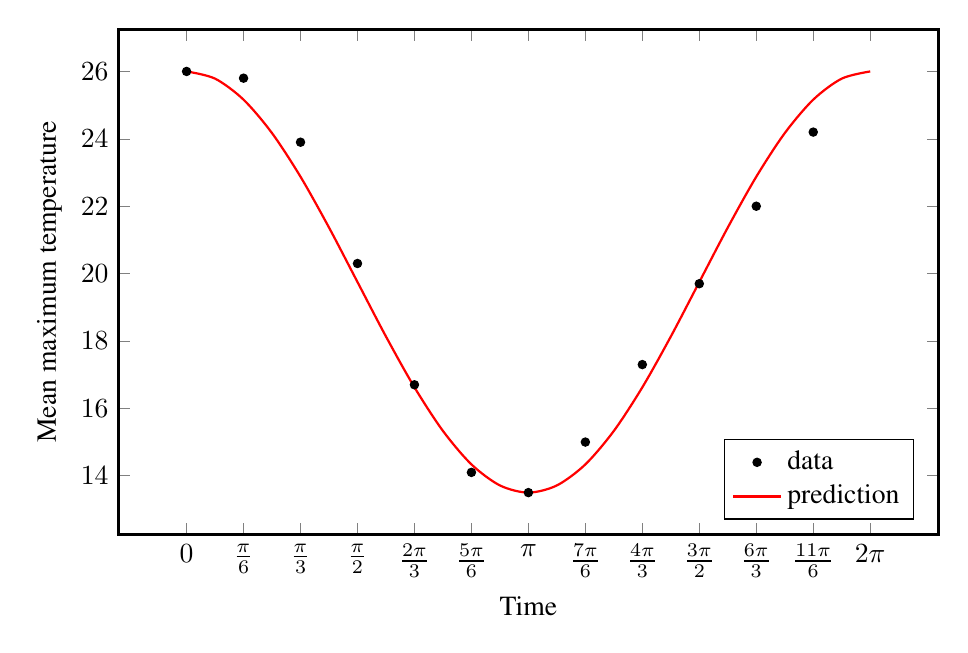
\begin{tikzpicture}
\tikzset{%%
  every mark/.append style={scale=1.0},%%
  scale=1.0%%
}
\pgfplotsset{%%
  every axis/.append style={font=\normalsize}%%
}
%%
\begin{axis}[%%
  axis line style=very thick,%%
  dotStyle/.style={mark size=1.5,black,mark color=black,mark=*,only marks},%%
  enlargelimits=true,%%
  height=8cm,%%
  legend cell align=left,%%
  legend pos=south east,%%
  plotStyle/.style={%%
    domain=0:2*pi,%%
    mark=none,%%
    smooth,%%
    thick%%
  },%%
  width=12cm,%%
  %% x axis
  xlabel={\normalsize Time},%%
  xtick={%%
    0,0.5236,1.0472,1.5708,2.0944,2.6179,3.1416,3.6652,4.1888,%%
    4.7124,5.2359,5.7596,6.2832%%
  },%%
  xticklabels={%%
    $0$,$\frac{\pi}{6}$,$\frac{\pi}{3}$,$\frac{\pi}{2}$,%%
    $\frac{2\pi}{3}$,$\frac{5\pi}{6}$,$\pi$,$\frac{7\pi}{6}$,%%
    $\frac{4\pi}{3}$,$\frac{3\pi}{2}$,$\frac{6\pi}{3}$,%%
    $\frac{11\pi}{6}$,$2\pi$%%
  },%%
  %% y axis
  ylabel={\normalsize Mean maximum temperature}%%
]
%%
%%
\addplot[dotStyle] coordinates {
  (0, 26)
  (0.523598775598299, 25.8)
  (1.0471975511966, 23.9)
  (1.5707963267949, 20.3)
  (2.0943951023932, 16.7)
  (2.61799387799149, 14.1)
  (3.14159265358979, 13.5)
  (3.66519142918809, 15)
  (4.18879020478639, 17.3)
  (4.71238898038469, 19.7)
  (5.23598775598299, 22)
  (5.75958653158129, 24.2)
};
\addlegendentry{data}
%%
%%
\addplot+ [plotStyle,red]
{6.25 * cos(deg(x)) + 19.75};
\addlegendentry{prediction}
\end{axis}
\end{tikzpicture}

\end{document}
